\documentclass[letterpaper,journal]{IEEEtran}

\usepackage{amsmath,amssymb}
\usepackage{algorithm}
\usepackage{algorithmic}
\usepackage{array}
\usepackage{booktabs}
\usepackage{cite}
\usepackage{graphicx}
\usepackage{placeins}
\usepackage{url}
\usepackage{tikz}
\usetikzlibrary{arrows.meta,positioning}

\graphicspath{{paper_assets/}}
\newcolumntype{L}[1]{>{\raggedright\arraybackslash}p{#1}}
\newcommand{\stdrel}{\operatorname{stdrel}}
\newcommand{\E}{\mathbb{E}}

\hyphenation{RMTGP ACOTSP phero-mone}

\begin{document}

\title{Residual Multi-Tree Genetic Programming for Joint Adaptation of State Transition and Pheromone Update Rules in Ant Colony Optimization}

\author{First Author, Second Author, and Third Author%
\thanks{Author names, affiliations, and funding information will be added after internal review.}}

\markboth{IEEE Transactions Draft, July 2026}%
{Author \MakeLowercase{\textit{et al.}}: Residual Multi-Tree Genetic Programming for ACO}

\maketitle

\begin{abstract}
Ant colony optimization depends on a state transition rule and a pheromone update rule.
Both rules are usually designed by experts.
Genetic programming can automate this design process.
However, direct replacement of a complete rule can remove useful structure from the original algorithm.
This study proposes residual multi-tree genetic programming for ant colony optimization, called RMTGP-ACO.
It uses two strongly typed trees.
The first tree applies a bounded correction to transition desirability.
The second tree redistributes pheromone deposits under a fixed event budget.
Zero output from both trees exactly recovers the original ACO.
We implement the method for Ant System, Ant Colony System, and MAX--MIN Ant System.
Training uses only uniform TSP100 instances.
Each ACO variant uses three independent genetic programming runs.
The selected programs are tested on uniform TSP50, TSP100, TSP500, and TSP1000.
Full-F1 reduces the mean reference gap in all 12 variant--scale comparisons.
The reduction ranges from 0.0736 to 7.8461 percentage points.
Controlled pilot ablations show that the residual effect depends on the ACO variant.
They do not show a stable benefit from the Full terminal set or the F1 function set.
Both evolved trees affect the selected programs, but pair-specific coadaptation is not stable.
All nine mean differences on the registered distribution-shift tests favor Full-F1.
Under a total budget of 31 nodes, the two-tree method does not consistently outperform both one-tree controls.
The 31/62-node capacity study remains ongoing.
A fused CUDA evaluator gives a 14.626-fold single-GPU speedup over a 16-thread CPU reference on the registered benchmark.
The results are a three-run pilot and are not confirmatory evidence.
\end{abstract}

\begin{IEEEkeywords}
Ant colony optimization, genetic programming, hyper-heuristic, multi-tree genetic programming, residual learning, traveling salesman problem.
\end{IEEEkeywords}

\section{Introduction}
\IEEEPARstart{A}{nt} colony optimization (ACO) constructs solutions from a pheromone model and problem-specific heuristic information \cite{dorigo1996antsystem,dorigo2004aco}.
Its behavior depends on two central components.
The state transition rule selects the next solution component.
The pheromone update rule changes the sampling model after each iteration.
These rules are effective, but they are usually fixed by human design.

Genetic programming (GP) can evolve executable rules \cite{koza1992gp,poli2008fieldguide}.
It can therefore reduce the need for manual formula design.
Previous GP-ACO work evolved complete state transition rules \cite{lin2025gpaco}.
That study showed that evolved rules can transfer across traveling salesman problem (TSP) sizes and distributions.
It also showed that global terminals can be useful.
However, a complete replacement changes the full transition model.
It does not preserve the original balance between pheromone and heuristic information.
It can also produce unstable score scales.

Pheromone adaptation creates a second design problem.
Earlier work used strongly typed GP to evolve pheromone strategies \cite{tavares2011pheromone}.
This direction is important, but joint transition and pheromone adaptation is difficult.
The two rules act at different points in ACO.
Their tensors also have different meanings and shapes.
A shared untyped tree would allow invalid combinations.
Two unrestricted trees would also receive more representational capacity than one tree.

We propose residual multi-tree genetic programming for ACO, or RMTGP-ACO.
The method uses one transition tree and one pheromone tree.
The trees have separate strong types.
The transition tree multiplies the original desirability by a bounded residual factor.
The pheromone tree redistributes a fixed deposit budget over the edges that the original ACO would reinforce.
The method retains the main semantics of Ant System (AS), Ant Colony System (ACS), and MAX--MIN Ant System (MMAS) \cite{dorigo1996antsystem,dorigo1997acs,stutzle2000mmas}.

This study makes four technical contributions.
\begin{itemize}
    \item It defines a bounded residual interface for ACO state transition.
    \item It defines an event-wise pheromone residual that preserves support and total deposit.
    \item It introduces a strongly typed two-tree representation with a shared node budget.
    \item It provides a fused GPU evaluator for the nested GP--ACO computation.
\end{itemize}

The current results form a three-run pilot.
They answer whether the complete method improves the original ACO.
They also provide controlled pilot evidence about the residual interface, tree roles, terminal and function profiles, and post-hoc coadaptation.
The 31/62-node capacity analysis is still ongoing.
We do not treat the current ablations as confirmatory causal evidence.

\section{Background and Problem Definition}

\subsection{Euclidean Traveling Salesman Problem}

Let \(V=\{1,\ldots,n\}\) be a set of cities.
Each city \(i\) has a coordinate \(c_i\in\mathbb{R}^2\).
The distance between cities \(i\) and \(j\) is
\begin{equation}
    d_{ij}=\lVert c_i-c_j\rVert_2.
\end{equation}
A tour is a permutation \(\pi=(\pi_1,\ldots,\pi_n)\).
Its length is
\begin{equation}
    L(\pi)=
    \sum_{q=1}^{n-1}d_{\pi_q,\pi_{q+1}}
    +d_{\pi_n,\pi_1}.
\end{equation}
The objective is to minimize \(L(\pi)\).

Each dataset row contains a reference tour.
We recompute its length in float64.
The available files do not provide a global optimality certificate for every tour.
We therefore use the term \emph{reference length}, denoted by \(L_i^{\mathrm{ref}}\).
The primary quality measure is
\begin{equation}
    g_i(\theta)
    =
    100
    \frac{L_i(\theta)-L_i^{\mathrm{ref}}}
    {L_i^{\mathrm{ref}}}.
    \label{eq:reference-gap}
\end{equation}
We call \(g_i\) the reference gap.

\subsection{Baseline ACO State Transition}

Let \(\tau_{ij}\) be the pheromone value of edge \((i,j)\).
Let
\begin{equation}
    \eta_{ij}=\frac{1}{d_{ij}+\epsilon_d}
\end{equation}
be its heuristic value.
At construction step \(q\), ant \(a\) is at city \(i\).
Its feasible set is \(F_{a,q}\).
The baseline desirability of city \(j\in F_{a,q}\) is
\begin{equation}
    s^0_{aij}=\tau_{ij}^{\alpha}\eta_{ij}^{\beta}.
    \label{eq:baseline-score}
\end{equation}

AS and MMAS sample from the normalized score.
ACS uses the pseudorandom proportional rule.
It selects the maximum score with probability \(q_0\).
Otherwise, it samples from the normalized score.
All variants use a candidate list.
If that list has no feasible city, the implementation uses the full feasible set.

\subsection{Baseline Pheromone Update}

AS evaporates all pheromone and reinforces the tours of all ants.
For ant \(a\), the baseline deposit on a tour edge is \(1/L_a\).
ACS applies its local update during construction.
It then applies a global update to the global-best tour.
MMAS reinforces one scheduled tour.
The schedule uses iteration-best tours and restart-best tours.
MMAS also applies dynamic pheromone bounds and restart logic.

Our implementation follows the algorithmic semantics of ACOTSP 1.03 \cite{stutzle2004acotsp}.
All three variants use 32 ants and 500 iterations in this study.
Local search is disabled.

\subsection{Previous GP-ACO Baseline}

The previous study evolved one complete state transition expression \cite{lin2025gpaco}.
We denote a matched implementation of that approach by Legacy-GP.
Its terminals are raw pheromone, raw distance, mean pheromone, mean distance, problem size, and feasible-set size.
It uses arithmetic primitives and a protected division that returns one when the denominator is close to zero.

The present study retrains Legacy-GP under the current data, ACO budget, and random schedules.
Published numerical results are not copied into the current paired tables.
This rule prevents a comparison between incompatible budgets.

\section{Residual Multi-Tree GP-ACO}

\subsection{Overview}

An RMTGP-ACO individual contains two programs:
\begin{equation}
    \theta=(T_{\mathrm{tr}},T_{\mathrm{ph}}).
\end{equation}
The transition program acts during solution construction.
The pheromone program acts after the colony tours are available.
Fig.~\ref{fig:framework} shows the data flow.

\begin{figure*}[t]
\centering
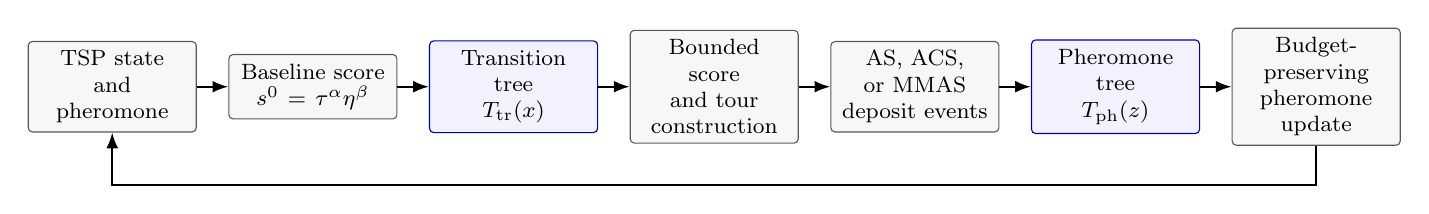
\begin{tikzpicture}[
    node distance=4mm and 4mm,
    box/.style={
        draw,
        rounded corners=1.5pt,
        align=center,
        minimum height=8mm,
        text width=19mm,
        font=\footnotesize
    },
    gpbox/.style={
        box,
        draw=blue!65!black,
        fill=blue!5
    },
    basebox/.style={
        box,
        draw=black!65,
        fill=black!3
    },
    arrow/.style={-{Latex[length=2mm]}, thick}
]
\node[basebox] (state) {TSP state\\and pheromone};
\node[basebox, right=of state] (basescore) {Baseline score\\\(s^0=\tau^\alpha\eta^\beta\)};
\node[gpbox, right=of basescore] (trtree) {Transition tree\\\(T_{\mathrm{tr}}(x)\)};
\node[basebox, right=of trtree] (construct) {Bounded score\\and tour construction};
\node[basebox, right=of construct] (events) {AS, ACS, or MMAS\\deposit events};
\node[gpbox, right=of events] (phtree) {Pheromone tree\\\(T_{\mathrm{ph}}(z)\)};
\node[basebox, right=of phtree] (update) {Budget-preserving\\pheromone update};

\draw[arrow] (state) -- (basescore);
\draw[arrow] (basescore) -- (trtree);
\draw[arrow] (trtree) -- (construct);
\draw[arrow] (construct) -- (events);
\draw[arrow] (events) -- (phtree);
\draw[arrow] (phtree) -- (update);
\draw[arrow] (update.south) -- ++(0,-5mm) -| (state.south);
\end{tikzpicture}
\caption{RMTGP-ACO data flow. The blue boxes are evolved programs. The other boxes retain the semantics of the selected ACO variant.}
\label{fig:framework}
\end{figure*}

\subsection{Strongly Typed Representation}

The implementation uses DEAP strongly typed GP
\cite{montana1995stgp,fortin2012deap}.
It defines two distinct Python marker classes:
\texttt{TrField} and \texttt{PhField}.
The two \texttt{PrimitiveSetTyped} root signatures are
\texttt{TRANSITION: () -> TrField} and
\texttt{PHEROMONE: () -> PhField}.
Every subtree inside one tree has the same field type as its root.
DEAP therefore rejects subtree exchange between the two semantic roles.

\begin{table*}[t]
\caption{Input, output, and execution location of the two typed GP trees}
\label{tab:strong-type}
\centering
\footnotesize
\renewcommand{\arraystretch}{1.15}
\resizebox{\textwidth}{!}{%
\begin{tabular}{L{25mm}L{30mm}L{40mm}L{43mm}L{30mm}}
\toprule
Tree & Strong type and shape & Dimension meaning & Input--output contract & Execution point\\
\midrule
Transition tree &
\texttt{TrField}, \([B,M,K]\) &
\(B\): ACO task batch; \(M\): ants; \(K\): current candidate width &
Maps a dynamic selection context to one candidate-level output field &
Every tour-construction step\\
Pheromone tree &
\texttt{PhField}, \([B,R,n]\) &
\(R\): reinforcement events; \(n\): edges in one closed tour &
Maps a dynamic reinforcement context to one event--edge output field &
Reinforcement stage of every ACO iteration\\
\bottomrule
\end{tabular}
}
\end{table*}

DEAP checks only the \texttt{TrField}/\texttt{PhField} marker during tree
construction, crossover, and mutation.
The shapes \([B,M,K]\) and \([B,R,n]\) are runtime contracts maintained by
the evaluator.
They are not additional DEAP static types.
This separation allows \(B,K,R,n\) to change with the batch, ACO variant,
and TSP size while preserving semantic type safety.

Each ACO task in \(B\) binds one program to one TSP instance.
When one individual is evaluated, \(B\) is the instance batch.
During fused population evaluation, \(B\) is the program--instance task batch.
Usually, \(K=\min(20,n-1)\).
Candidate-list fallback uses \(K=n\).
AS has \(R=M=32\).
ACS has \(R=1\) and uses the global-best source tour.
MMAS has \(R=1\) and retains its original reinforcement schedule.

\begin{table*}[t]
\caption{Runtime context available to each tree in one call}
\label{tab:runtime-context}
\centering
\footnotesize
\renewcommand{\arraystretch}{1.15}
\setlength{\tabcolsep}{4pt}
\begin{tabular}{L{28mm}L{73mm}L{67mm}}
\toprule
Context & Raw information and shape & Meaning of one output element\\
\midrule
Transition &
Distance \(d\), heuristic \(\eta\), and pheromone \(\tau\):
\([B,n,n]\);
current city \(c\): \([B,M]\);
candidate city \(C\) and feasible mask \(F\): \([B,M,K]\);
baseline probability \(p^0\): \([B,M,K]\);
construction step \(q\), ACO iteration \(t\), budget \(T\), and
stagnation counter \(s[B]\) &
\(X^{\mathrm{tr}}_{bak}\) is one terminal value for task \(b\), ant \(a\),
and candidate slot \(k\).
\(C_{bak}\) maps that slot to a city.\\
Pheromone reinforcement &
\(d,\eta,\tau\), and full nearest-neighbor rank: \([B,n,n]\);
source tour \(\pi^{\mathrm{src}}\): \([B,R,n+1]\);
expanded endpoints \(u,v\): \([B,R,n]\);
source length: \([B,R]\);
colony tours: \([B,M,n+1]\);
colony lengths: \([B,M]\);
\(t,T\), and \(s[B]\) &
\(X^{\mathrm{ph}}_{bre}\) is one terminal value for edge position \(e\)
of reinforcement event \(r\) in task \(b\).\\
\bottomrule
\end{tabular}
\end{table*}

The empty argument list in each root signature does not mean that a tree has
no information.
Each named terminal is a zero-arity typed leaf that is bound to the current
ACO context at runtime.
The evaluator constructs only terminals that are referenced by the program.
The PyTorch backend can materialize the full fields.
The fused CUDA and Numba backends compute the same logical values in flattened
or compact form.
The reported shapes are therefore logical tensor shapes.
They do not require every terminal to be materialized at the same time.

If a fused call evaluates \(P\) deduplicated programs on \(I\) instances,
then \(B=PI\).
For TSP100 with \(M=32\) and \(K=20\), the transition field is
\([PI,32,20]\).
The AS pheromone field is \([PI,32,100]\).
The ACS and MMAS pheromone fields are \([PI,1,100]\).

The two trees share one fitness.
They also share a total size limit:
\begin{equation}
    N_{\mathrm{tr}}+N_{\mathrm{ph}}\leq 31.
    \label{eq:node-budget}
\end{equation}
An inactive zero tree has zero effective nodes.
Each tree also has a maximum depth of five.
Equation~\eqref{eq:node-budget} is the active constraint in the main study.
The two trees therefore share 31 effective nodes in total.
The limit is not 31 nodes per tree.
This rule prevents a two-tree individual from receiving twice the capacity
of a one-tree individual.

\subsection{Transition Residual}

The transition tree receives the terminal field \(x_{aij}\).
Its raw output is
\begin{equation}
    u_{aij}=T_{\mathrm{tr}}(x_{aij}).
\end{equation}
The output changes the baseline score in \eqref{eq:baseline-score}:
\begin{align}
    r_{aij} &= \tanh(u_{aij}),\\
    m_{aij} &= 1+\gamma_{\mathrm{tr}}r_{aij},\\
    \widetilde{s}_{aij} &= s^0_{aij}m_{aij},
    \label{eq:transition-residual}
\end{align}
where \(\gamma_{\mathrm{tr}}=1/3\).
The final probability is
\begin{equation}
    p_{aij}
    =
    \frac{\widetilde{s}_{aij}}
    {\sum_{\ell\in F_{a,q}}\widetilde{s}_{ai\ell}}.
\end{equation}

This interface has four useful properties.
First, a zero tree gives \(m_{aij}=1\).
It exactly recovers the baseline ACO.
Second, \(m_{aij}\in[2/3,4/3]\).
The score remains positive.
Third, infeasible edges remain infeasible.
Fourth, for two feasible cities \(j\) and \(k\),
\begin{equation}
    \frac{m_{aij}}{m_{aik}}\in[1/2,2].
\end{equation}
The tree can change a local preference, but it cannot create an unbounded score ratio.

\subsection{Pheromone Residual}

A deposit event is
\begin{equation}
    r=(\pi_r,L_r,w_r).
\end{equation}
\(\pi_r\) is a source tour.
\(L_r\) is its length.
\(w_r\) is the baseline weight.
For each edge \(e\) in \(\pi_r\), the baseline deposit is
\begin{equation}
    D^0_{r,e}=\frac{w_r}{L_r}.
\end{equation}
The total event budget is
\begin{equation}
    B_r=\sum_{e\in E(\pi_r)}D^0_{r,e}
       =\frac{nw_r}{L_r}.
\end{equation}

The pheromone tree produces
\begin{align}
    v_{r,e} &= T_{\mathrm{ph}}(z_{r,e}),\\
    h_{r,e} &= 1+\gamma_{\mathrm{ph}}\tanh(v_{r,e}),
\end{align}
where \(\gamma_{\mathrm{ph}}=1/3\).
The final deposit is
\begin{equation}
    \widetilde{D}_{r,e}
    =
    B_r
    \frac{D^0_{r,e}h_{r,e}}
    {\sum_{f\in E(\pi_r)}D^0_{r,f}h_{r,f}}.
    \label{eq:pheromone-residual}
\end{equation}

The zero tree recovers the baseline deposit.
The reinforced edge set is unchanged.
The event budget is also conserved:
\begin{equation}
    \sum_{e\in E(\pi_r)}\widetilde{D}_{r,e}=B_r.
\end{equation}
AS creates one event for each ant.
ACS creates one global-best event.
MMAS creates one event from its original update schedule.
The residual only redistributes each event.
It does not modify ACS local updates, MMAS bounds, or MMAS restart decisions.

\subsection{Residual Strength}

Both interfaces use the same residual strength, \(\gamma=1/3\).
In general, the multiplier is
\begin{equation}
    m(y)=1+\gamma\tanh(y),
    \qquad
    1-\gamma\leq m(y)\leq1+\gamma.
    \label{eq:residual-radius}
\end{equation}
Any \(\gamma<1\) preserves a positive multiplier.
For \(\gamma=1/3\), one multiplier is bounded by \(2/3\) and \(4/3\).
The ratio between the multipliers of two candidates is at most two.
After probability or deposit-share normalization, an original share can change
by at most a factor from \(1/2\) to \(2\).
This range allows GP to change a relative preference while retaining the
baseline rule as the dominant component.

The value \(1/3\) was fixed before the test results were inspected.
It was not selected on a test set.
A value of \(0.1\) would allow only a weak correction.
A value of \(0.5\) would allow a threefold relative correction between two
candidates.
We use the same value for both trees to remove one potential confounder.
The current ablation does not treat \(\gamma\) as a factor.
A future sensitivity study can compare \(0.1\), \(1/3\), and \(0.5\).

\subsection{Terminal Design Principles}

The basic terminals in the previous GP-ACO study were pheromone concentration
and distance \cite{lin2025gpaco}.
Its extended configuration also included mean candidate pheromone, mean
candidate distance, the number of cities, and the number of unvisited cities.
Those terminals are suitable when GP must generate a complete transition score.
We do not copy that set unchanged because the present trees learn residuals.
The baseline score \(s^0=\tau^\alpha\eta^\beta\) already preserves the main
absolute relation between pheromone and distance.
The residual tree does not need to reconstruct that relation.

\begin{table*}[t]
\caption{Relation between the previous GP-ACO terminals and the present design}
\label{tab:terminal-comparison}
\centering
\footnotesize
\renewcommand{\arraystretch}{1.15}
\setlength{\tabcolsep}{3pt}
\begin{tabular}{L{39mm}L{59mm}L{70mm}}
\toprule
Previous input & Corresponding information in this study & Design reason\\
\midrule
Pheromone concentration and distance &
\texttt{RTau}, \texttt{REta}, and the retained baseline score \(s^0\) &
The ACO absolute score structure is retained.
The tree observes relative strength inside the current candidate set.\\
Mean candidate pheromone and mean candidate distance &
Within-group normalization of \texttt{RTau}/\texttt{REta}, plus
\texttt{BaseConf} and \texttt{Entropy} &
Location and scale enter the normalization.
The latter terminals directly describe concentration of the baseline choice
distribution.\\
Number of cities and number of unvisited cities &
\texttt{ConstructProg}, \texttt{DistRank}, and \texttt{NNRank} &
Ratios and ranks replace raw counts.
Their ranges do not grow linearly with TSP size.\\
No pheromone-update-specific inputs &
\texttt{EdgeEta}, \texttt{EdgeTau}, \texttt{ColonyFreq}, and
\texttt{SourceQuality} &
The second tree acts on reinforcement events.
It requires edge quality, colony agreement, and source-tour quality.\\
\bottomrule
\end{tabular}
\end{table*}

Table~\ref{tab:terminal-comparison} maps information roles.
It does not claim algebraic equivalence between the two terminal sets.
We remove absolute means and raw city counts because they shift with the
pheromone stage and problem size.
The baseline ACO state still retains their effects.
Our hypothesis is that relative inputs transfer more easily across sizes.
Legacy-GP compares the two overall representations, but it cannot isolate one
terminal.

The design follows four rules.
First, every terminal must be available at decision time.
Reference tours and reference lengths are never terminal inputs.
Second, continuous inputs use relative values, ranks, or progress ratios when
possible.
Third, the set covers local edge quality, baseline confidence, search stage,
and colony feedback.
Fourth, the terminal count must support a controlled Core/Full ablation.
We do not assume that Full is better.
The Core/Full comparison tests the group-level increment.
It does not prove that Core is minimal or identify the causal effect of one
terminal.

\subsection{Transition Terminal Set}

Many raw ACO values depend on the problem size and iteration.
The main terminal set uses bounded relative values.
For a vector \(y\) and its active mask, define
\begin{equation}
    \stdrel(y)
    =
    \tanh\left(
    \frac{y-\operatorname{mean}(y)}
    {\operatorname{std}(y)+\epsilon}
    \right).
    \label{eq:stdrel}
\end{equation}
The mean and standard deviation are computed over the last active dimension.
Masked entries receive zero.

\begin{table*}[t]
\caption{Runtime inputs, calculation, and logical tensor shape of transition terminals}
\label{tab:transition-terminals}
\centering
\scriptsize
\renewcommand{\arraystretch}{1.18}
\setlength{\tabcolsep}{2.5pt}
\begin{tabular}{L{20mm}L{31mm}L{49mm}L{58mm}L{14mm}}
\toprule
Terminal & Type; native shape \(\to\) tree-input shape &
Information read from the ACO state & Calculation and candidate-axis meaning &
Profile\\
\midrule
\texttt{RTau} &
\texttt{TrField};
\([B,M,K]\to[B,M,K]\) &
\(\tau[B,n,n]\), current city \([B,M]\), candidate city and feasible mask
\([B,M,K]\) &
Gather pheromone from the current city to each candidate.
Normalize \(\log(\max(\tau,\epsilon))\) over the feasible \(K\) axis of each
task--ant pair, then apply \(\tanh\). &
Core, Full\\
\texttt{REta} &
\texttt{TrField};
\([B,M,K]\to[B,M,K]\) &
\(\eta[B,n,n]\), current city \([B,M]\), candidate city and feasible mask
\([B,M,K]\) &
Gather the heuristic value for each candidate.
Apply log normalization over the feasible \(K\) axis and then \(\tanh\). &
Core, Full\\
\texttt{BaseConf} &
\texttt{TrField};
\([B,M,K]\to[B,M,K]\) &
\(\tau,\eta,\alpha,\beta\), feasible mask, and
\(p^0[B,M,K]\) from \(s^0=\tau^\alpha\eta^\beta\) &
For feasible count \(k\), compute
\(\tanh[\log(p^0+\epsilon)+\log k]\) for each candidate.
A uniform distribution maps to zero. &
Core, Full\\
\texttt{DistRank} &
\texttt{TrField};
\([B,M,K]\to[B,M,K]\) &
Distance matrix \(d[B,n,n]\), current city, candidate city, and feasible mask &
Rank candidates by distance within each feasible \(K\) set.
Map rank \(r\) to \(1-2(r-1)/(k-1)\).
Use zero when \(k=1\). &
Core, Full\\
\texttt{Entropy} &
\texttt{TrField};
\([B,M,1]\to[B,M,K]\) &
Baseline probability \(p^0[B,M,K]\), feasible mask, and feasible count
\(k[B,M,1]\) &
Compute \(2H(p^0)/\log k-1\) over \(K\), then broadcast to all candidates.
Use \(-1\) when \(k=1\). &
Full\\
\texttt{ConstructProg} &
\texttt{TrField};
\([1]\to[B,M,K]\) &
Current construction step \(q\) and city count \(n\) &
Compute \(2q/\max(n-1,1)-1\), then broadcast over \(B,M,K\). &
Full\\
\texttt{ACOProg} &
\texttt{TrField};
\([1]\to[B,M,K]\) &
Current ACO iteration \(t\) and total iterations \(T\) &
Compute \(2(t-1)/\max(T-1,1)-1\), then broadcast to all ants and candidates. &
Full\\
\texttt{Stagnation} &
\texttt{TrField};
\([B,1,1]\to[B,M,K]\) &
Task-level non-improvement count \(s_t[B]\) and \(T\) &
Compute \(2\min(s_t/T,1)-1\), then broadcast over ants and candidates. &
Full\\
\bottomrule
\end{tabular}
\end{table*}

\texttt{RTau} and \texttt{REta} describe the relative strength of the two
baseline ACO signals.
\texttt{BaseConf} describes confidence in one candidate.
\texttt{DistRank} gives scale-insensitive local geometric order.
These four terminals form Core.
\texttt{Entropy} describes ambiguity of the complete choice distribution.
\texttt{ConstructProg}, \texttt{ACOProg}, and \texttt{Stagnation} describe
search context.
They enlarge the search space and therefore belong only to Full.

\subsection{Pheromone Terminal Set}

Each value in Table~\ref{tab:pheromone-terminals} corresponds to one edge in
one reinforcement event.
The runtime context includes source tours
\(\pi^{\mathrm{src}}[B,R,n+1]\), their lengths
\(L^{\mathrm{src}}[B,R]\), colony tours
\(\pi^{\mathrm{col}}[B,M,n+1]\), and colony lengths
\(L^{\mathrm{col}}[B,M]\).
Each source tour is expanded to endpoints \(u,v[B,R,n]\).
Every terminal therefore enters the tree as
\texttt{PhField} \([B,R,n]\).
An event scalar is broadcast over the edge axis.
A task scalar is broadcast over both the event and edge axes.

\begin{table*}[t]
\caption{Runtime inputs, calculation, and logical tensor shape of pheromone terminals}
\label{tab:pheromone-terminals}
\centering
\scriptsize
\renewcommand{\arraystretch}{1.18}
\setlength{\tabcolsep}{2.5pt}
\begin{tabular}{L{20mm}L{31mm}L{49mm}L{58mm}L{14mm}}
\toprule
Terminal & Type; native shape \(\to\) tree-input shape &
Information read from the ACO state & Calculation and event--edge meaning &
Profile\\
\midrule
\texttt{EdgeEta} &
\texttt{PhField};
\([B,R,n]\to[B,R,n]\) &
\(\eta[B,n,n]\), endpoints \(u,v[B,R,n]\), and candidate-neighborhood mean
\(\log\eta[B,n]\) for each city &
Subtract the mean endpoint neighborhood value from edge \(\log\eta_{uv}\).
Normalize over the \(n\) edges of each task--event pair and apply \(\tanh\). &
Core, Full\\
\texttt{EdgeTau} &
\texttt{PhField};
\([B,R,n]\to[B,R,n]\) &
\(\tau[B,n,n]\) and endpoints \(u,v[B,R,n]\) &
Gather \(\tau_{uv}\) for every source edge.
Normalize \(\log(\max(\tau_{uv},\epsilon))\) over the \(n\) edges of each event
and apply \(\tanh\). &
Core, Full\\
\texttt{NNRank} &
\texttt{PhField};
\([B,R,n]\to[B,R,n]\) &
Precomputed full nearest-neighbor ranks \([B,n,n]\) and endpoints
\(u,v[B,R,n]\) &
Map the directed ranks \(u\!\to\!v\) and \(v\!\to\!u\) by
\(1-2(r-1)/\max(n-2,1)\), then average the two directions. &
Core, Full\\
\texttt{ColonyFreq} &
\texttt{PhField};
\([B,R,n]\to[B,R,n]\) &
Current colony tours \(\pi^{\mathrm{col}}[B,M,n+1]\) and source endpoints
\(u,v\) &
Ignore direction and count how many of the \(M\) colony tours contain each
source edge.
Compute \(2c_e/M-1\). &
Full\\
\texttt{SourceQuality} &
\texttt{PhField};
\([B,R,1]\to[B,R,n]\) &
Source length \(L^{\mathrm{src}}[B,R]\) and colony lengths
\(L^{\mathrm{col}}[B,M]\) &
Compute colony mean \(\overline L\) and population standard deviation
\(\sigma_L\) over \(M\).
Use \(\tanh[(\overline L-L^{\mathrm{src}}_r)/(\sigma_L+\epsilon)]\), then
broadcast over the \(n\) edges. &
Core, Full\\
\texttt{ACOProg} &
\texttt{PhField};
\([1]\to[B,R,n]\) &
Current ACO iteration \(t\) and total iterations \(T\) &
Compute \(2(t-1)/\max(T-1,1)-1\), then broadcast to all events and edges. &
Full\\
\texttt{Stagnation} &
\texttt{PhField};
\([B,1,1]\to[B,R,n]\) &
Task-level non-improvement count \(s_t[B]\) and \(T\) &
Compute \(2\min(s_t/T,1)-1\), then broadcast over events and edges. &
Full\\
\bottomrule
\end{tabular}
\end{table*}

\texttt{EdgeEta}, \texttt{EdgeTau}, and \texttt{NNRank} describe the reinforced
edge.
\texttt{SourceQuality} describes the route that produced that edge.
These four terminals form Core.
\texttt{ColonyFreq}, \texttt{ACOProg}, and \texttt{Stagnation} add colony and
search-stage context.
They belong only to Full.

Both primitive sets also contain the constants
\(-1,-0.5,0,0.5,1\).
They contain one ephemeral random constant sampled from \(U[-1,1]\).
An ERC mutation adds Gaussian noise with standard deviation \(0.1\).
The result is clipped to \([-1,1]\).
The constants are also strongly typed terminals.
A transition constant returns \texttt{TrField}.
A pheromone constant returns \texttt{PhField}.
The evaluator broadcasts a constant to \([B,M,K]\) or \([B,R,n]\).
There is no untyped scalar terminal that can cross the two roles.

\subsection{Function Sets and Numerical Protection}

Table~\ref{tab:functions} gives the two function profiles.
All operations are element-wise.
F1 extends F0.
Protected division is
\begin{equation}
    \operatorname{PDIV}(x,y)
    =
    \frac{xy}{y^2+10^{-6}}.
    \label{eq:pdiv}
\end{equation}
This form is continuous at \(y=0\).
After each primitive, NaN is replaced by zero.
Positive and negative infinity are replaced by \(10\) and \(-10\).
Every result is then clipped to \([-10,10]\).
The external residual interface applies another \(\tanh\).

\begin{table*}[t]
\caption{GP function set and strongly typed input--output signatures}
\label{tab:functions}
\centering
\footnotesize
\renewcommand{\arraystretch}{1.16}
\setlength{\tabcolsep}{4pt}
\begin{tabular}{L{18mm}L{38mm}L{55mm}L{35mm}L{18mm}}
\toprule
Function & Calculation & Input type & Output type & Profile\\
\midrule
\texttt{ADD} & \(x+y\) &
\texttt{TrField}\(\times\)\texttt{TrField} or
\texttt{PhField}\(\times\)\texttt{PhField} &
\texttt{TrField} or \texttt{PhField} & F0, F1\\
\texttt{SUB} & \(x-y\) &
\texttt{TrField}\(\times\)\texttt{TrField} or
\texttt{PhField}\(\times\)\texttt{PhField} &
\texttt{TrField} or \texttt{PhField} & F0, F1\\
\texttt{MUL} & \(xy\) &
\texttt{TrField}\(\times\)\texttt{TrField} or
\texttt{PhField}\(\times\)\texttt{PhField} &
\texttt{TrField} or \texttt{PhField} & F0, F1\\
\texttt{PDIV} & \(xy/(y^2+10^{-6})\) &
\texttt{TrField}\(\times\)\texttt{TrField} or
\texttt{PhField}\(\times\)\texttt{PhField} &
\texttt{TrField} or \texttt{PhField} & F0, F1\\
\texttt{NEG} & \(-x\) &
\texttt{TrField} or \texttt{PhField} &
\texttt{TrField} or \texttt{PhField} & F0, F1\\
\texttt{MIN} & \(\min(x,y)\) &
\texttt{TrField}\(\times\)\texttt{TrField} or
\texttt{PhField}\(\times\)\texttt{PhField} &
\texttt{TrField} or \texttt{PhField} & F1\\
\texttt{MAX} & \(\max(x,y)\) &
\texttt{TrField}\(\times\)\texttt{TrField} or
\texttt{PhField}\(\times\)\texttt{PhField} &
\texttt{TrField} or \texttt{PhField} & F1\\
\texttt{ABS} & \(|x|\) &
\texttt{TrField} or \texttt{PhField} &
\texttt{TrField} or \texttt{PhField} & F1\\
\bottomrule
\end{tabular}
\end{table*}

Each function is registered twice.
For example, transition \texttt{ADD} has signature
\((\texttt{TrField},\texttt{TrField})\to\texttt{TrField}\).
Pheromone \texttt{ADD} has signature
\((\texttt{PhField},\texttt{PhField})\to\texttt{PhField}\).
One call cannot mix the two types.

Legacy-GP uses ADD, SUB, MUL, NEG, and \(\operatorname{PDIV1}\).
Its protected division returns \(x/y\) when \(|y|>10^{-6}\).
It returns one otherwise.
Matched-Replace uses the Full terminals and F1.
Its raw transition output becomes a positive score through
\begin{equation}
    s_{aij}=\operatorname{softplus}(\operatorname{clip}(u_{aij},-20,20))+\epsilon.
\end{equation}

F0 can form smooth low-order combinations.
F1 adds simple piecewise rules through \texttt{MIN}, \texttt{MAX}, and
\texttt{ABS}.
We omit exponential, logarithmic, and trigonometric primitives.
The terminals already include log transformations and bounded normalization.
The residual interface also applies \(\tanh\).
Adding these functions would enlarge the equivalent-expression space and
increase numerical risk.
We also omit explicit conditional branches.
\texttt{MIN} and \texttt{MAX} provide simple gating and are easier to fuse.
The F0/F1 factor tests whether the additional functions are necessary.

\subsection{Evolutionary Search}

The initial joint population contains four modes.
Ten percent are exact baseline sentinels.
Twenty percent activate only the transition tree.
Twenty percent activate only the pheromone tree.
The remaining 50 percent activate both trees.
Active trees use ramped half-and-half initialization with depths from two to four.

Elitism keeps the best ten individuals.
The remaining offspring use crossover with probability \(0.80\), mutation with probability \(0.15\), and reproduction with probability \(0.05\).
Tournament size is four.
Crossover selects one active role and applies typed one-point crossover within that role.
Mutation selects one active role.
It uses subtree mutation with probability \(0.50\), node replacement with probability \(0.30\), and ERC perturbation with probability \(0.20\).
An offspring that violates the depth or node limit is replaced by its valid parent.

Structural hashes avoid repeated evaluation within one generation.
The GPU evaluator also groups programs with identical compiled behavior.
These operations do not change the fitness.

For a training set \(\mathcal{I}\) and ACO seed set \(\mathcal{S}\), fitness is
\begin{equation}
    F(\theta)
    =
    \frac{1}{|\mathcal{I}||\mathcal{S}|}
    \sum_{i\in\mathcal{I}}
    \sum_{s\in\mathcal{S}}
    g_{i,s}(\theta).
    \label{eq:fitness}
\end{equation}
The objective minimizes the absolute reference gap.
It does not minimize a baseline-relative value.
It contains no parsimony penalty.
Program size is used only to break defined ties.
For reporting, we separately define
\begin{equation}
    \Delta g=g_{\mathrm{method}}-g_{\mathrm{ACO}}.
    \label{eq:delta}
\end{equation}
A negative \(\Delta g\) favors the learned method.

\begin{algorithm}[t]
\caption{One RMTGP-ACO simulation}
\label{alg:rmtgp-aco}
\begin{algorithmic}[1]
\REQUIRE TSP instance, ACO variant, \(T_{\mathrm{tr}}\), \(T_{\mathrm{ph}}\)
\STATE Initialize pheromone and variant-specific search state
\FOR{\(t=1,\ldots,T\)}
    \FOR{each construction step \(q\)}
        \STATE Build the active candidate set
        \STATE Compute baseline score \(s^0=\tau^\alpha\eta^\beta\)
        \STATE Build only the terminals used by \(T_{\mathrm{tr}}\)
        \STATE Apply the bounded residual in \eqref{eq:transition-residual}
        \STATE Select cities with the original variant rule
        \STATE Apply the ACS local update when required
    \ENDFOR
    \STATE Compute all tour lengths and update best states
    \STATE Build AS, ACS, or MMAS deposit events
    \STATE Build only the terminals used by \(T_{\mathrm{ph}}\)
    \STATE Apply the budget residual in \eqref{eq:pheromone-residual}
    \STATE Apply variant evaporation, bounds, and restart logic
\ENDFOR
\RETURN Best tour; recompute its length in CPU float64
\end{algorithmic}
\end{algorithm}

\begin{algorithm}[t]
\caption{GP training and champion selection}
\label{alg:gp-training}
\begin{algorithmic}[1]
\REQUIRE Frozen training and validation schedules
\STATE Load or create immutable baseline ACO archives
\STATE Initialize 100 typed two-tree individuals
\FOR{\(h=1,\ldots,50\)}
    \STATE Load 32 scheduled TSP100 training instances
    \STATE Use one shared ACO seed for all individuals
    \STATE Evaluate unique programs and assign \eqref{eq:fitness}
    \STATE Save the top five every five generations
    \STATE Create the next population with typed operators
\ENDFOR
\STATE Screen unique checkpoints on 32 selection instances with one seed
\STATE Re-evaluate the best five with three paired seeds
\STATE Find the minimum mean gap
\STATE Within 0.01 percentage points, select the smaller program
\STATE Audit this candidate on 32 disjoint gate instances
\RETURN One selected candidate and one gate-deployed policy
\end{algorithmic}
\end{algorithm}

\section{Experimental Methodology}

\subsection{Research Questions}

Table~\ref{tab:rq} lists the seven research questions and the available
evidence.
RQ1, RQ2, and RQ4--RQ6 have complete three-run pilot quality results.
The 31-node part of RQ3 is complete.
The 31/62-node capacity study is ongoing.
The fused training benchmark in RQ7 is complete, while some isolated
single-program timing cells are ongoing.

\begin{table*}[t]
\caption{Research questions, primary comparisons, and current status}
\label{tab:rq}
\centering
\footnotesize
\renewcommand{\arraystretch}{1.15}
\begin{tabular}{L{11mm}L{63mm}L{70mm}L{20mm}}
\toprule
Question & Research question & Primary comparison & Status\\
\midrule
RQ1 & Does Full-F1 reduce the reference gap of the original ACO? &
Full-F1 versus the corresponding AS, ACS, or MMAS baseline & Complete\\
RQ2 & Is residual transition adaptation better than complete transition
replacement? &
TR-RGP versus Matched-Replace & Complete\\
RQ3 & Under the same total node budget, is a two-tree method better than a
one-tree method? &
Full-F1 versus independently trained TR-RGP and PH-RGP &
B31 complete; capacity ongoing\\
RQ4 & Does the improvement depend on Full terminals or F1 functions? &
Core/Full \(\times\) F0/F1 factorial experiment & Complete\\
RQ5 & Is there joint coadaptation between the two trees? &
Tree deletion and cross-run tree-pair shuffling & Complete\\
RQ6 & Does a TSP100-trained program transfer across sizes and distributions? &
TSP50/500/1000, cluster, Gaussian, and TSPLIB & Complete\\
RQ7 & How much acceleration does the fused implementation provide? &
CPU8, CPU16, one GPU, two-GPU shard, and parallel campaign &
Training complete; deployment timing ongoing\\
\bottomrule
\end{tabular}
\end{table*}

\subsection{Data}

The training pool contains 1,280,000 uniform TSP100 instances.
It consists of ten files with 128,000 instances each.
A frozen schedule selects 32 different instances per generation.
One GP run therefore sees \(32\times50=1,600\) different training instances.
The full pool is much larger than the consumed subset.
This design supports independent schedules for additional GP runs.

The validation file contains 1,280 uniform TSP100 instances.
Each GP run uses 32 instances for selection and 32 disjoint instances for the non-inferiority gate.
The completed test sets contain 1,280 uniform TSP50 instances, 1,280 uniform TSP100 instances, 128 uniform TSP500 instances, and 128 uniform TSP1000 instances.
TSP1000 is a locked-model supplementary extrapolation set.
It is not used during evolution or model selection.

The registered distribution tests contain 128 clustered TSP500 instances, 128 Gaussian TSP500 instances, and 42 TSPLIB instances with \(n\leq500\) \cite{reinelt1991tsplib}.
They are used only for the locked Full-F1 champions.
No program is selected again on these partitions.
All files are identified by a manifest and a SHA-256 checksum.
Train, validation, and test coordinates remain separated.
Reference-tour edges are never used as GP terminals.

\begin{table}[t]
\caption{Data used by the TSP100 pilot}
\label{tab:data}
\centering
\footnotesize
\begin{tabular}{llr}
\toprule
Role & Partition & Instances\\
\midrule
Training pool & TSP100 uniform & 1,280,000\\
Per GP run & \(32\times50\) TSP100 & 1,600\\
Validation & Selection / gate & \(32/32\)\\
Test & TSP50 uniform & 1,280\\
Test & TSP100 uniform & 1,280\\
Test & TSP500 uniform & 128\\
Test & TSP1000 uniform & 128\\
OOD test & TSP500 cluster / Gaussian & \(128/128\)\\
OOD test & TSPLIB, \(n\leq500\) & 42\\
\bottomrule
\end{tabular}
\end{table}

\subsection{Compared Methods and Ablations}

Table~\ref{tab:methods} maps each method to its scientific purpose.
Full-F1 is the proposed main configuration.
Core and Full refer to the terminal sets in Tables~\ref{tab:transition-terminals} and \ref{tab:pheromone-terminals}.
F0 and F1 refer to Table~\ref{tab:functions}.

\begin{table*}[t]
\caption{Methods, controlled differences, and current result status}
\label{tab:methods}
\centering
\footnotesize
\renewcommand{\arraystretch}{1.15}
\begin{tabular}{L{22mm}L{24mm}L{24mm}L{24mm}L{42mm}L{15mm}}
\toprule
Method & Transition integration & Pheromone integration & Terminal/function profile & Main purpose & Status\\
\midrule
Baseline ACO & None & None & None & Original AS, ACS, or MMAS & Complete\\
Legacy-GP & Full replacement & None & Legacy & Prior GP-ACO structure under the current budget & Complete\\
Matched-Replace & Full replacement & None & Full/F1 & Replacement control for RQ2 & Complete\\
TR-RGP & Residual & None & Full/F1 & Independent transition-only control & Complete\\
PH-RGP & None & Budget residual & Full/F1 & Independent pheromone-only control & Complete\\
RMTGP Core-F0 & Residual & Budget residual & Core/F0 & Factorial terminal/function control & Complete\\
RMTGP Core-F1 & Residual & Budget residual & Core/F1 & Factorial terminal/function control & Complete\\
RMTGP Full-F0 & Residual & Budget residual & Full/F0 & Factorial terminal/function control & Complete\\
RMTGP Full-F1 & Residual & Budget residual & Full/F1 & Proposed main method & Complete\\
Drop and shuffle & Post-hoc intervention & Post-hoc intervention & Frozen Full/F1 trees & Coadaptation analysis for RQ5 & Complete\\
\bottomrule
\end{tabular}
\end{table*}

RQ2 uses TR-RGP minus Matched-Replace as its primary estimand.
Legacy-GP is a secondary methodological baseline.
RQ3 compares Full-F1 with independently trained TR-RGP and PH-RGP.
All three methods first use a total node budget of 31.
A separate capacity study compares budgets of 31 and 62.
RQ4 uses a \(2\times2\) factorial design.
It estimates the terminal main effect, the function main effect, and their interaction.
RQ5 drops each tree and shuffles independently evolved tree pairs.
The post-hoc interventions complement the independent one-tree controls.
They do not replace them.

\subsection{ACO and GP Parameters}

Table~\ref{tab:parameters} gives the common parameters.
AS uses \(\rho=0.5\).
ACS uses \(\rho=0.1\), \(q_0=0.9\), and \(\xi=0.1\).
MMAS uses \(\rho=0.02\).
Its update period is 25.
Its \(p_{\mathrm{best}}\) value is 0.05.
Its branch check period is 100.
Its branch parameter is 0.05.
Its branch threshold is 1.00001.
Its restart stagnation limit is 250.
ACS applies synchronous local updates.

\begin{table}[t]
\caption{Common experimental parameters}
\label{tab:parameters}
\centering
\footnotesize
\begin{tabular}{ll}
\toprule
Parameter & Value\\
\midrule
ACO ants & 32\\
ACO iterations & 500\\
Candidate-list size & 20\\
\(\alpha,\beta\) & \(1,2\)\\
\(\gamma_{\mathrm{tr}},\gamma_{\mathrm{ph}}\) & \(1/3,1/3\)\\
Local search & Disabled\\
GP population & 100\\
GP generations & 50\\
Crossover / mutation / reproduction & \(0.80/0.15/0.05\)\\
Elites / tournament size & \(10/4\)\\
Initial depth / maximum depth & \(2\)--\(4/5\)\\
Total effective node budget & 31\\
Checkpoint interval / retained count & \(5/5\)\\
Training instances per generation & 32\\
Selection / gate instances & \(32/32\)\\
Screening / final validation seeds & \(1/3\)\\
Test ACO seeds per instance & 3\\
Independent GP runs per variant & 3\\
CPU threads / process count & \(16/1\)\\
CUDA block threads & 32\\
Search / final score precision & FP32 / FP64\\
\bottomrule
\end{tabular}
\end{table}

The GP root seeds are 1001--1003 for AS, 2001--2003 for ACS, and 3001--3003 for MMAS.
Final test seeds are derived from a separate root seed of 9001.
They are independent of the GP seeds.
All methods within a paired comparison share the same instances and ACO seeds.

\subsection{Champion Selection and Reported Policy}

Each generation uses one ACO seed.
All individuals share that seed and the same 32 instances.
This pairing reduces within-generation noise.
The baseline ACO values are precomputed and stored in immutable archives.

The validation procedure first screens checkpoints with one seed.
It then evaluates the five best checkpoints with three seeds.
It selects the smallest tree among candidates within 0.01 percentage points of the best mean gap.
Only this selected individual enters the independent gate.
The gate accepts a candidate when the one-sided 95\% upper bound of its validation delta is at most 0.10 percentage points.

The main scientific analysis uses the selected candidate from each GP run.
It retains all three GP runs.
It does not select the best GP seed.
The gate-deployed policy is a separate operational quantity.
It falls back to baseline ACO when a candidate fails the gate.

\subsection{Statistical Analysis}

The primary response is the reference gap in \eqref{eq:reference-gap}.
We also record worst-decile conditional value at risk, anytime gap area under the curve, best iteration, wall time, and win/tie/loss rates.
A win means that the learned method has a smaller gap than its paired baseline.

The three ACO seeds are first averaged within an instance.
The main statistical block is then GP-run by instance.
We use a paired Wilcoxon signed-rank test \cite{wilcoxon1945}.
Holm correction is applied within each ACO variant and RQ family \cite{holm1979}.
We also use a hierarchical bootstrap \cite{efron1994bootstrap}.
It resamples GP runs, then instances, then ACO seeds.
Each interval uses 10,000 replicates.

Only three GP runs are available in this pilot.
This count is too small for a final claim about evolutionary-run uncertainty.
The confidence intervals and tests are therefore descriptive.
A confirmatory study will use 30 independent GP runs.

\subsection{Evolution Curves and Final-Test Protocol}

The training curve does not use the median fitness of the population.
For each independent GP run and generation, we first select the individual
with minimum fitness.
Program size breaks an exact fitness tie.
The training point is the mean reference gap of that generation-best
individual on the 32 new training instances.
Because every generation uses a different batch, short-term changes are not
strict estimates of generalization.

The validation point evaluates the same generation-best individual on the
fixed 32 selection instances and the fixed screening seed.
It is not the population median or the best-so-far validation value.
For each ACO variant, the plotted line is the median of the three independent
GP runs at the same generation.
The band is their minimum and maximum.
The baseline line uses the same fixed validation instances and seed.

The final test does not use the last-generation individual directly.
The candidate pool contains the top five individuals from every fifth
generation and the top five from the last generation.
Duplicate structures are removed.
Screening, three-seed reevaluation, and the independent gate select one
champion for each GP run.
All three champions enter the scientific test.
The test sets are used only for final measurement.

\section{Efficient Implementation}

\subsection{Batched Evaluation Architecture}

The nested fitness is expensive.
One population contains 100 individuals.
Each individual invokes ACO on 32 instances.
Each ACO invocation constructs \(32\times500\) tours.
A direct Python loop over individuals, instances, ants, and iterations is not practical.

The implementation uses NumPy, Numba, PyTorch, DEAP, and CuPy \cite{harris2020numpy,lam2015numba,paszke2019pytorch,fortin2012deap,okuta2017cupy}.
The CPU backend forms a population-by-instance task matrix.
Numba compiles the inner ACO loops.
The GPU backend goes further.
It compiles each typed GP tree to a compact postfix program.
It removes structurally and behaviorally duplicate programs.
It then forms a program-by-instance task grid.

One CUDA block owns one program--instance task.
Thirty-two threads match the 32 ants.
The block performs all 500 ACO iterations.
It evaluates both GP programs inside the kernel.
It also performs candidate fallback, ACS local-update multiplicities, MMAS bounds, and MMAS restart logic.
Problem tensors and terminal-independent features remain resident on the device.
A counter-based random generator makes task partitioning deterministic.

The GPU searches in FP32.
It returns the best tour.
The host recomputes that tour length from the original float64 distance matrix.
The final fitness and all paper tables therefore use CPU FP64 tour scoring.

\subsection{Parallel Scheduling}

One GP run uses one process and one visible GPU.
Population-level and instance-level work are fused inside the kernel.
This design avoids multiple Python processes competing for one GPU.
Independent GP runs are the main multi-GPU unit.
They are assigned to different devices.
This campaign mode maximizes aggregate throughput.

A dual-shard mode can split one generation over two GPUs.
It reduces the latency of one run.
Its scaling is weaker because each shard is smaller.
The registered scheduler therefore uses independent runs when enough runs are available.
CPU16 remains the deterministic fallback and the FP64 audit backend.

\subsection{Formal Acceleration Benchmark}

The formal benchmark used an Intel Xeon W-2245 CPU and two 20-GiB NVIDIA RTX 4000 Ada Generation GPUs.
The workload used ACS, 100 requested individuals, 79 behaviorally unique programs, 16 TSP50 instances, 16 TSP100 instances, 32 ants, and 500 ACO iterations.
One workload constructed 40,448,000 tours.
Each mode used one cold run and three warm runs.
Table~\ref{tab:speed} reports the warm median.

\begin{table}[t]
\caption{Formal accelerator benchmark}
\label{tab:speed}
\centering
\footnotesize
\begin{tabular}{lrrr}
\toprule
Mode & Time (s) & Tours/s & CPU16 ratio\\
\midrule
CPU8 & 397.422 & 101,776 & 0.766\\
CPU16 & 304.325 & 132,911 & 1.000\\
GPU0 & 20.807 & 1,943,957 & 14.626\\
GPU1 & 20.838 & 1,941,110 & 14.605\\
Dual shard & 12.776 & 3,165,928 & 23.820\\
Campaign$^\dagger$ & 21.101 & 3,833,840 & 28.9\\
\bottomrule
\multicolumn{4}{l}{\scriptsize $^\dagger$Two concurrent workloads; ratio uses aggregate throughput.}
\end{tabular}
\end{table}

\begin{figure}[t]
\centering
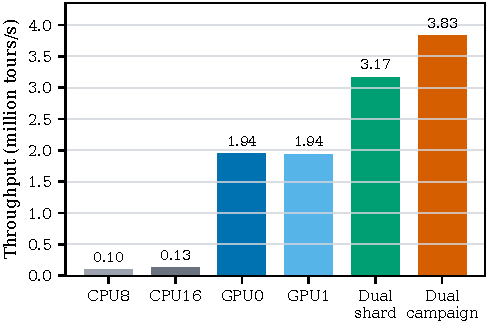
\includegraphics[width=\columnwidth]{accelerator_throughput.pdf}
\caption{Throughput on the formal accelerator benchmark. Campaign throughput is aggregated over two concurrent workloads.}
\label{fig:throughput}
\end{figure}

Single-run dual-GPU scaling is \(20.807/12.776=1.629\).
Concurrent campaign scaling is \(2(20.807)/21.101=1.972\).
The first value is below the registered 1.7 scaling gate.
The second value is above the registered 1.8 campaign gate.
This result supports task-level multi-GPU scheduling.

Average GPU utilization was about 99\%.
Peak device memory was about 286 MiB.
About 99.8\% of warm time was inside the CUDA kernel.
The workload was compute-bound.
Additional memory caching is therefore unlikely to be the main source of future speedup.

The numerical quality audit used TSP50 and TSP100.
It used 128 instances per size and three paired ACO seeds.
Let \(\Delta_{\mathrm{num}}=g_{\mathrm{GPU}}-g_{\mathrm{CPU}}\).
The pooled mean was \(-0.003445\) percentage points.
The one-sided 95\% upper bound was \(0.000868\) percentage points.
This value is below the registered 0.10 threshold.

The observed mean generation times are shown in Table~\ref{tab:generation-time}.
They include all unique population evaluations for one generation.
They do not include final test evaluation.

\begin{table}[t]
\caption{Observed generation time across three GP runs}
\label{tab:generation-time}
\centering
\footnotesize
\begin{tabular}{lrr}
\toprule
Variant & Mean \(\pm\) SD (s) & Run range (s)\\
\midrule
% 本文件由 build_paper_assets.py 生成，请勿手工修改。
AS & 34.50 $\pm$ 2.97 & 31.13--36.78 \\
ACS & 26.88 $\pm$ 4.43 & 21.97--30.57 \\
MMAS & 22.14 $\pm$ 3.34 & 18.31--24.41 \\
\bottomrule
%
\end{tabular}
\end{table}

\section{Results and Analysis}

\subsection{RQ1: Full-F1 Versus Baseline ACO}

Table~\ref{tab:main-results} reports the completed selected-candidate results.
The baseline column contains the original ACO gap.
The Full-F1 column contains the learned-method gap.
The confidence interval is for \(\Delta g\).
Negative values favor Full-F1.

\begin{table*}[t]
\caption{Selected-candidate results on completed uniform test sets. CI denotes the hierarchical bootstrap 95\% interval of \(\Delta g\). W/T/L is reported in percent.}
\label{tab:main-results}
\centering
\footnotesize
\renewcommand{\arraystretch}{1.12}
\begin{tabular}{lrrrrrl}
\toprule
ACO & \(n\) & Baseline gap (\%) & Full-F1 gap (\%) & \(\Delta g\) (pp) & 95\% CI (pp) & W/T/L\\
\midrule
% 本文件由 build_paper_assets.py 生成，请勿手工修改。
AS & 50 & 1.8803 & 1.7479 & -0.1324 & [-0.2076, -0.0718] & 54.7/2.8/42.4 \\
AS & 100 & 5.8952 & 4.2154 & -1.6799 & [-1.9680, -1.4739] & 92.1/0.0/7.9 \\
AS & 500 & 22.9874 & 15.1413 & -7.8461 & [-8.3979, -7.3727] & 100.0/0.0/0.0 \\
AS & 1000 & 30.4224 & 23.1088 & -7.3135 & [-8.5940, -6.1418] & 100.0/0.0/0.0 \\
ACS & 50 & 0.7326 & 0.6589 & -0.0736 & [-0.1050, -0.0432] & 46.6/17.6/35.9 \\
ACS & 100 & 1.9331 & 1.6412 & -0.2918 & [-0.3954, -0.2091] & 64.7/0.0/35.3 \\
ACS & 500 & 16.1641 & 12.9399 & -3.2242 & [-4.5698, -1.3932] & 93.8/0.0/6.2 \\
ACS & 1000 & 21.6293 & 19.2041 & -2.4252 & [-3.3961, -0.8317] & 94.8/0.0/5.2 \\
MMAS & 50 & 0.5941 & 0.4727 & -0.1215 & [-0.1549, -0.0820] & 52.3/22.4/25.2 \\
MMAS & 100 & 4.1088 & 1.8106 & -2.2982 & [-2.4240, -2.1223] & 99.2/0.0/0.8 \\
MMAS & 500 & 20.6291 & 14.1769 & -6.4522 & [-8.1652, -4.7067] & 100.0/0.0/0.0 \\
MMAS & 1000 & 25.4885 & 18.8571 & -6.6314 & [-8.3746, -4.8120] & 100.0/0.0/0.0 \\
\bottomrule
%
\end{tabular}
\end{table*}

\begin{figure*}[t]
\centering
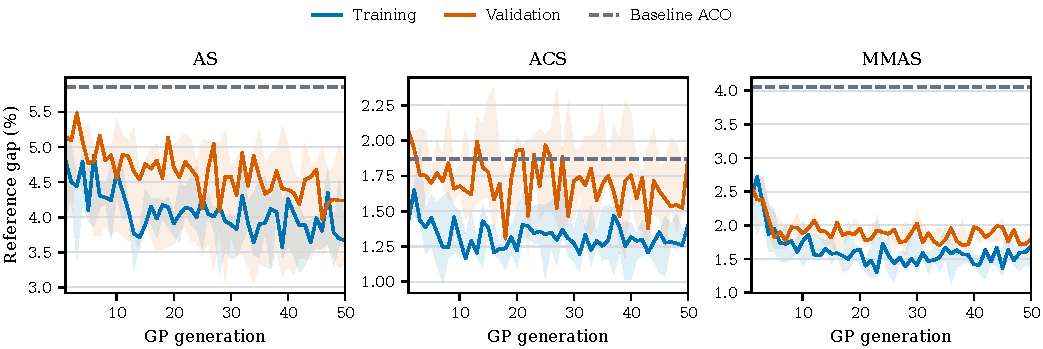
\includegraphics[width=\textwidth]{training_validation_curves.pdf}
\caption{TSP100 training and validation curves.
For each run, a training point is the generation-best individual on that
generation's new batch.
The validation point evaluates the same individual on the fixed selection set.
Lines are medians over three independent GP runs.
Bands show their minimum and maximum.}
\label{fig:training-curves}
\end{figure*}

\begin{figure*}[t]
\centering
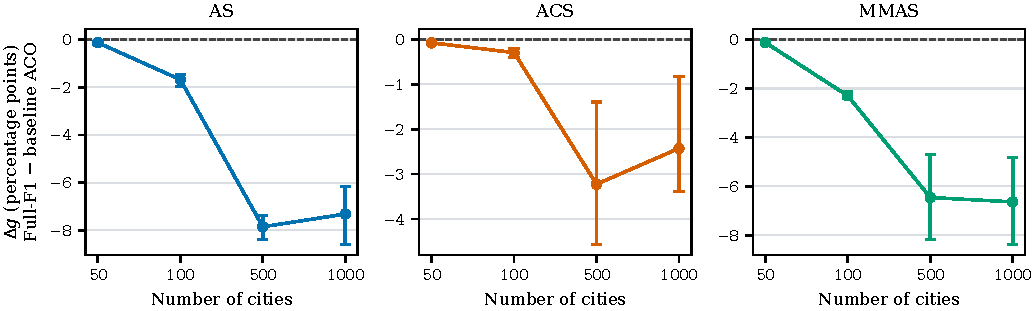
\includegraphics[width=\textwidth]{main_gap_delta.pdf}
\caption{Full-F1 minus baseline ACO reference gap. Error bars are hierarchical bootstrap 95\% intervals. Negative values favor Full-F1.}
\label{fig:main-delta}
\end{figure*}

All 12 mean differences are negative.
All 12 bootstrap intervals are below zero.
The smallest observed reduction is 0.0736 percentage points for ACS on TSP50.
The largest reduction is 7.8461 percentage points for AS on TSP500.
The Holm-adjusted Wilcoxon values are at most \(9.004\times10^{-17}\).
These test values describe the current blocks.
They do not replace replication over more GP runs.

AS improves from 1.8803\% to 1.7479\% on TSP50.
It improves from 5.8952\% to 4.2154\% on TSP100.
Its reductions are larger on TSP500 and TSP1000.
They are 7.8461 and 7.3135 percentage points.

ACS has smaller gains at the two smaller sizes.
Its reduction is 0.2918 percentage points on TSP100.
It reaches 3.2242 percentage points on TSP500.
One of the three ACS candidates did not pass the independent deployment gate.
The selected-candidate table retains that run because the analysis must not remove an unfavorable GP replicate.
The operational gate-deployed result is therefore weaker than the selected-candidate result for ACS.

MMAS improves from 4.1088\% to 1.8106\% on TSP100.
Its reductions are 6.4522 and 6.6314 percentage points on TSP500 and TSP1000.
Its TSP100 win rate is 99.2\%.
Its TSP500 and TSP1000 win rates are 100\% in the current blocks.

Fig.~\ref{fig:training-curves} shows noisy training curves.
This behavior is expected because every generation uses a new batch.
The validation curves are also not monotonic.
The selected checkpoint can therefore differ from the last generation.
The independent selection procedure is necessary.

\begin{figure*}[t]
\centering
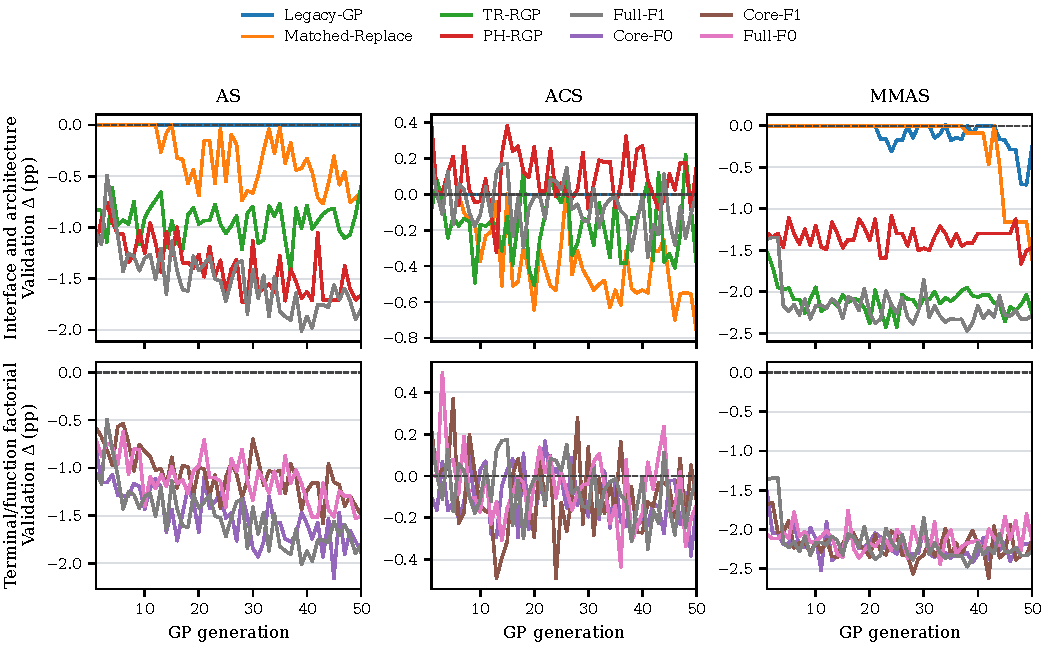
\includegraphics[width=\textwidth]{ablation_validation_curves.pdf}
\caption{Validation-delta curves for all ablation methods on the fixed
selection set.
Each line is the median of three GP runs at the same generation.
The upper row compares integration interfaces and tree structures.
The lower row compares Core/Full \(\times\) F0/F1.
Negative values are below the original ACO.}
\label{fig:ablation-validation-curves}
\end{figure*}

Fig.~\ref{fig:ablation-validation-curves} uses the same validation protocol.
The curves diagnose evolution only.
Final comparisons use independently selected champions and locked test sets.
A zero tree is a valid individual.
A zero-delta plateau for Legacy-GP therefore means that a zero tree won that
generation; it is not missing data.

\textbf{Answer to RQ1:}
Full-F1 has a lower mean reference gap than the corresponding original ACO in every completed pilot comparison.
This is evidence for effectiveness.
It is not yet evidence that the residual interface, two-tree structure, or Full/F1 primitive profile is the cause.

\subsection{RQ2: Residual Versus Full Replacement}

\begin{table}[!t]
\caption{Paired residual-versus-replacement differences.
Each cell is the mean difference [95\% hierarchical bootstrap interval] in
percentage points.
Negative values favor the residual interface.}
\label{tab:residual-effects}
\centering
\scriptsize
\setlength{\tabcolsep}{2.5pt}
\resizebox{\columnwidth}{!}{%
\begin{tabular}{llr}
\toprule
ACO & Test & TR-RGP \(-\) Matched-Replace\\
\midrule
% 自动生成；负值表示 residual 接口具有更低 gap。
AS & TSP100-U & -0.606 [-0.853, -0.413] \\
AS & TSP500-U & -2.558 [-3.119, -1.720] \\
ACS & TSP100-U & +0.311 [+0.216, +0.436] \\
ACS & TSP500-U & +5.430 [+3.726, +6.602] \\
MMAS & TSP100-U & -0.679 [-1.224, +0.291] \\
MMAS & TSP500-U & -1.706 [-3.790, +0.452] \\
\bottomrule
%
\end{tabular}}
\end{table}

\begin{figure}[!t]
\centering
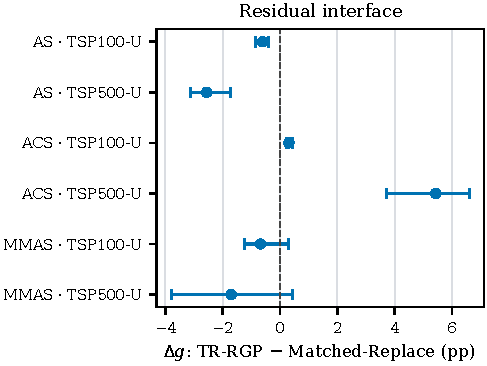
\includegraphics[width=\columnwidth]{residual_effects.pdf}
\caption{Paired residual-versus-replacement differences.
Error bars are 95\% hierarchical bootstrap intervals.
Negative values favor residual integration.}
\label{fig:residual-effects}
\end{figure}

Table~\ref{tab:residual-effects} and Fig.~\ref{fig:residual-effects} give the
direct RQ2 estimand.
TR-RGP and Matched-Replace both use one transition tree.
They share the Full terminals, F1 functions, 31-node budget, training data,
and random schedule.
Only the integration interface changes.

Both AS intervals are below zero.
The estimates are \(-0.6058\) and \(-2.5584\) percentage points.
Both ACS intervals are above zero.
The estimates are \(+0.3114\) and \(+5.4303\) percentage points.
Both MMAS means are negative, at \(-0.6795\) and \(-1.7058\), but both
intervals cross zero.
Thus, two of six contexts support residual integration.
Two support complete replacement.
Two favor residual integration in direction only.

MMAS pheromone bounds and the residual interface both limit a deviation.
They do not act on the same variable.
MMAS clips updated pheromone.
RQ2 changes the candidate transition score.
The two mechanisms should therefore not be treated as equivalent.
The present MMAS intervals also do not show a clear residual advantage.

Legacy-GP changes the terminal and function sets together with the interface.
It is an auxiliary prior-work baseline and cannot isolate the residual effect.

\textbf{Answer to RQ2:}
The pilot does not support a universal residual advantage.
Residual integration is better for AS.
Complete replacement is better for ACS.
The MMAS evidence is uncertain.

\subsection{RQ3: Two Trees Versus One Tree}

\subsubsection{Architecture at a Fixed 31-Node Budget}

\begin{table}[!t]
\caption{Paired differences between the two-tree method and independently
trained one-tree methods under a total 31-node budget.
Each cell is the mean difference [95\% hierarchical bootstrap interval] in
percentage points.
Negative values favor the two-tree method.}
\label{tab:architecture-b31}
\centering
\scriptsize
\setlength{\tabcolsep}{2.5pt}
\resizebox{\columnwidth}{!}{%
\begin{tabular}{llrr}
\toprule
ACO & Test & Full-F1 \(-\) TR-RGP & Full-F1 \(-\) PH-RGP\\
\midrule
% 自动生成；负值表示 31 节点双树具有更低 gap。
AS & TSP100-U & -0.525 [-0.876, -0.265] & -0.068 [-0.230, +0.100] \\
AS & TSP500-U & -0.994 [-1.580, -0.153] & +0.795 [+0.597, +1.007] \\
ACS & TSP100-U & -0.006 [-0.179, +0.113] & -0.263 [-0.393, -0.167] \\
ACS & TSP500-U & +0.304 [-1.843, +2.336] & -2.950 [-4.575, -1.219] \\
MMAS & TSP100-U & -0.056 [-0.182, +0.144] & -0.828 [-0.970, -0.659] \\
MMAS & TSP500-U & -0.810 [-2.601, +1.187] & -1.162 [-3.075, +0.731] \\
\bottomrule
%
\end{tabular}}
\end{table}

\begin{figure}[!t]
\centering
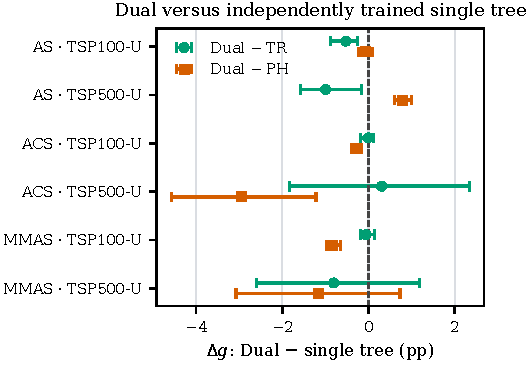
\includegraphics[width=\columnwidth]{architecture_effects.pdf}
\caption{Two-tree versus independently trained one-tree differences under a
total 31-node budget.
Error bars are 95\% hierarchical bootstrap intervals.
Negative values favor the two-tree method.}
\label{fig:architecture-b31}
\end{figure}

Table~\ref{tab:architecture-b31} and Fig.~\ref{fig:architecture-b31} compare
Full-F1, TR-RGP, and PH-RGP.
All three methods are trained independently.
All three share 31 total effective nodes.
The two-tree method divides that total between its two trees.

Full-F1 has two intervals below zero relative to TR-RGP.
The other four intervals cross zero.
No interval clearly favors TR-RGP.
Relative to PH-RGP, Full-F1 has three intervals below zero, two intervals
crossing zero, and one AS/TSP500 interval above zero.
No context simultaneously shows that Full-F1 is better than both one-tree
methods.

\subsubsection{31/62-Node Capacity Sensitivity}

This experiment is ongoing.
It retrains TR-RGP, PH-RGP, and Full-F1.
A one-tree method can use 62 nodes at \(B=62\).
The two-tree method shares 62 total nodes at \(B=62\).
This design separates the number of semantic roles from total expression
capacity.
Deleting one tree from an existing Full-F1 individual does not replace this
independent training control.

\textbf{Current answer to RQ3:}
At a total budget of 31 nodes, the pilot does not show that two trees
consistently outperform both one-tree controls.
The capacity study is required to determine whether this result is caused by
the total node limit.

\subsection{RQ4: Terminal and Function Profiles}

\begin{table*}[!t]
\caption{Core/Full \(\times\) F0/F1 factorial effects.
Each cell is the mean contrast [95\% hierarchical bootstrap interval] in
percentage points.}
\label{tab:factorial-effects}
\centering
\scriptsize
\setlength{\tabcolsep}{3pt}
\resizebox{\textwidth}{!}{%
\begin{tabular}{llrrr}
\toprule
ACO & Test & Full \(-\) Core & F1 \(-\) F0 &
\((\mathrm{Full\mbox{-}F1}-\mathrm{Full\mbox{-}F0})
-(\mathrm{Core\mbox{-}F1}-\mathrm{Core\mbox{-}F0})\)\\
\midrule
% 自动生成；负值表示相应线性 contrast 降低 gap。
AS & TSP100-U & -0.213 [-0.534, +0.021] & +0.501 [-0.254, +0.990] & -0.410 [-0.900, +0.406] \\
AS & TSP500-U & -0.414 [-1.433, +0.844] & +0.951 [+0.066, +2.504] & -1.953 [-5.492, +1.437] \\
ACS & TSP100-U & -0.030 [-0.122, +0.071] & -0.022 [-0.058, +0.016] & -0.005 [-0.063, +0.057] \\
ACS & TSP500-U & +0.210 [-1.043, +2.296] & -0.219 [-1.197, +0.373] & +0.074 [-0.383, +0.548] \\
MMAS & TSP100-U & +0.085 [+0.017, +0.155] & +0.033 [-0.042, +0.143] & -0.004 [-0.215, +0.186] \\
MMAS & TSP500-U & +0.528 [+0.080, +1.163] & +0.353 [-1.106, +1.365] & +0.549 [-1.514, +2.519] \\
\bottomrule
%
\end{tabular}}
\end{table*}

\begin{figure*}[!t]
\centering

\includegraphics[width=\textwidth]{factorial_effects.pdf}
\caption{Terminal main effect, function main effect, and their interaction.
Negative values indicate a reduction in reference gap.
Error bars are 95\% hierarchical bootstrap intervals.}
\label{fig:factorial-effects}
\end{figure*}

The factorial experiment contains Core-F0, Core-F1, Full-F0, and Full-F1.
The average Full-minus-Core difference is the terminal main effect.
The average F1-minus-F0 difference is the function main effect.
The difference in these differences is the interaction.

No Full-minus-Core interval is below zero.
Four intervals cross zero.
The MMAS TSP100 and TSP500 intervals are above zero and favor Core.
No F1-minus-F0 interval is below zero.
Five intervals cross zero.
The AS TSP500 interval is above zero and favors F0.
All six interaction intervals cross zero.

\begin{figure}[t]
\centering
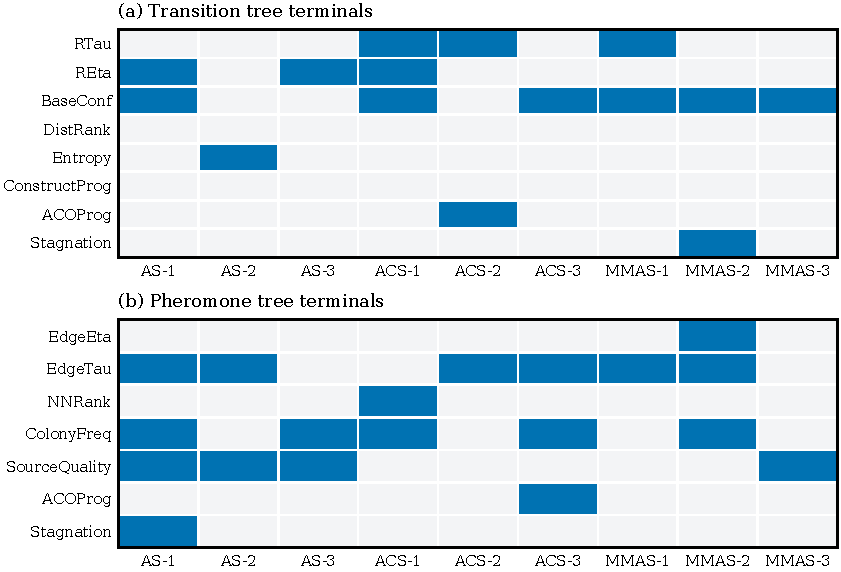
\includegraphics[width=\columnwidth]{terminal_usage_heatmap.pdf}
\caption{Syntactic terminal use by the nine Full-F1 champions.
Blue indicates that an expression references a terminal at least once.
The plot does not test whether a reference remains active after algebraic
simplification.}
\label{fig:terminal-usage}
\end{figure}

Fig.~\ref{fig:terminal-usage} provides a syntax audit.
\texttt{BaseConf} appears in 6/9 transition champions.
\texttt{DistRank} and \texttt{ConstructProg} appear in none.
\texttt{Entropy}, \texttt{ACOProg}, and \texttt{Stagnation} each appear once.
For pheromone trees, \texttt{EdgeTau} appears in 6/9 champions and
\texttt{ColonyFreq} appears in 5/9.
\texttt{ACOProg} and \texttt{Stagnation} each appear once.
Syntactic occurrence is not causal contribution.
A terminal can appear in a canceled subexpression.

\textbf{Answer to RQ4:}
The pilot does not show a stable benefit from the Full terminal set or the F1
additions.
Three contexts instead support a simpler profile.
The current Full/F1 design may therefore be over-specified.
The Full-F1 main results remain valid, but a confirmatory study should
prioritize Core-F0 or Core-F1.

\subsection{RQ5: Joint Coadaptation}

\begin{table*}[!t]
\caption{Post-training component deletion and cross-run pairing interventions
for Full-F1.
Each cell is the mean difference [95\% hierarchical bootstrap interval] in
percentage points.
Negative values favor the original Full-F1 pair.}
\label{tab:mechanism-effects}
\centering
\scriptsize
\setlength{\tabcolsep}{2.5pt}
\resizebox{\textwidth}{!}{%
\begin{tabular}{llrrrr}
\toprule
ACO & Test & Full \(-\) drop-TR & Full \(-\) drop-PH &
Full \(-\) shuffle-r1 & Full \(-\) shuffle-r2\\
\midrule
% 自动生成；负值表示原始 Full-F1 配对更好。
AS & TSP100-U & -0.270 [-0.728, +0.000] & -1.290 [-1.576, -1.058] & -0.214 [-0.349, -0.097] & -0.292 [-0.735, +0.211] \\
AS & TSP500-U & -1.824 [-5.132, +0.000] & -6.090 [-7.765, -3.058] & -0.666 [-5.459, +2.957] & -0.749 [-5.407, +3.422] \\
ACS & TSP100-U & -0.273 [-0.321, -0.222] & -0.018 [-0.091, +0.048] & -0.032 [-0.092, +0.039] & -0.007 [-0.147, +0.121] \\
ACS & TSP500-U & -2.817 [-4.044, -0.854] & -0.341 [-0.659, -0.019] & -0.116 [-0.598, +0.273] & -0.236 [-0.540, +0.110] \\
MMAS & TSP100-U & -1.534 [-2.102, -1.006] & -0.134 [-0.255, +0.000] & +0.014 [-0.254, +0.239] & +0.026 [-0.135, +0.250] \\
MMAS & TSP500-U & -4.403 [-4.679, -4.140] & -1.551 [-2.834, +0.000] & -0.027 [-1.769, +2.845] & -0.029 [-2.834, +1.633] \\
\bottomrule
%
\end{tabular}}
\end{table*}

\begin{figure*}[!t]
\centering
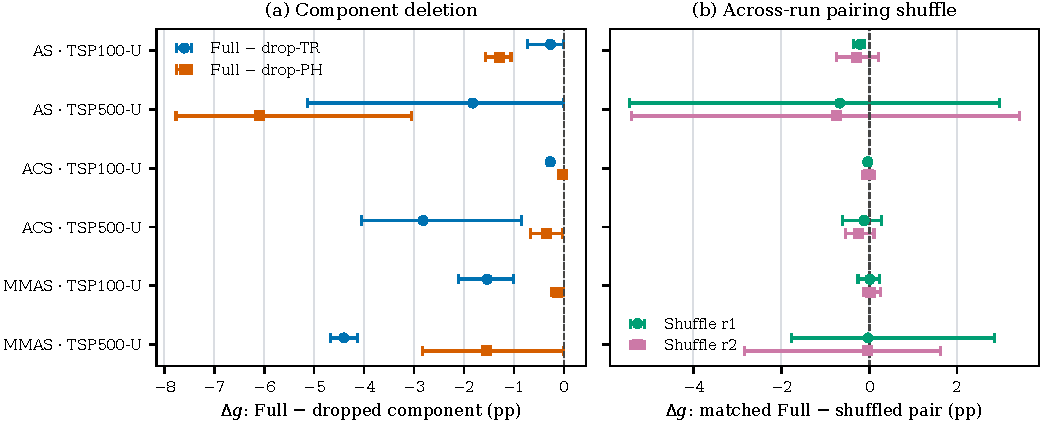
\includegraphics[width=\textwidth]{mechanism_effects.pdf}
\caption{Post-training tree deletion and cross-run tree-pair shuffling.
Negative values favor the original Full-F1 champion.
Error bars are 95\% hierarchical bootstrap intervals.}
\label{fig:mechanism-effects}
\end{figure*}

The first intervention replaces the transition tree with zero.
The second replaces the pheromone tree with zero.
All six Full-minus-drop-TR means are negative.
Four intervals are strictly below zero.
The other two have an upper bound of zero.
The transition tree is therefore usually necessary for the selected
champions.

Full-minus-drop-PH is also mainly negative.
Three intervals are strictly below zero.
Two have an upper bound of zero.
One crosses zero.
The pheromone tree also contributes, but its evidence is less consistent.

The third intervention shuffles the two trees across independent GP runs.
Only the AS/TSP100 r1 interval is below zero among the 12 shuffle intervals.
The other 11 cross zero.
The current data therefore do not show a stable advantage for the original
within-run pairing.

\textbf{Answer to RQ5:}
Both components affect the selected Full-F1 individuals.
The transition-tree effect is more consistent.
The pilot does not show stable pair-specific coadaptation.
This post-hoc result does not replace the independently trained one-tree
controls in RQ3.

\FloatBarrier

\subsection{RQ6: Generalization}

The uniform results support scale transfer.
Training and validation use only TSP100.
TSP50, TSP500, and TSP1000 are unseen sizes.
All nine ACO-variant--unseen-size mean differences are negative.
The absolute reduction is generally larger at TSP500 and TSP1000.

\begin{table*}[!t]
\caption{Descriptive distribution-shift results.
W/T/L is the percentage over GP-run--instance blocks.
The table is not used for causal claims about terminals or functions.}
\label{tab:ood-results}
\centering
\footnotesize
\begin{tabular}{llrrrl}
\toprule
ACO & Test & Baseline gap (\%) & Full-F1 gap (\%) &
\(\Delta g\) (pp) & W/T/L\\
\midrule
% 自动生成；OOD 不进行 terminal/function 因果推断。
AS & TSP500-C & 26.0627 & 19.7383 & -6.3245 & 100.0/0.0/0.0 \\
AS & TSP500-G & 20.0986 & 14.0184 & -6.0802 & 100.0/0.0/0.0 \\
AS & TSPLIB$\leq$500 & 10.0277 & 7.6313 & -2.3964 & 82.5/0.0/17.5 \\
ACS & TSP500-C & 16.3527 & 13.8345 & -2.5182 & 90.6/0.0/9.4 \\
ACS & TSP500-G & 14.8973 & 12.6798 & -2.2175 & 88.3/0.0/11.7 \\
ACS & TSPLIB$\leq$500 & 4.5376 & 3.5976 & -0.9399 & 77.8/0.0/22.2 \\
MMAS & TSP500-C & 22.7375 & 16.5961 & -6.1414 & 100.0/0.0/0.0 \\
MMAS & TSP500-G & 17.6609 & 12.1975 & -5.4635 & 100.0/0.0/0.0 \\
MMAS & TSPLIB$\leq$500 & 8.3755 & 5.0336 & -3.3419 & 93.7/2.4/4.0 \\
\bottomrule
%
\end{tabular}
\end{table*}

\begin{figure}[t]
\centering
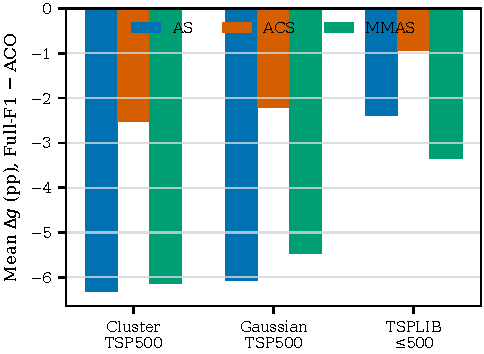
\includegraphics[width=\columnwidth]{ood_delta.pdf}
\caption{Descriptive mean differences on cluster, Gaussian, and TSPLIB
partitions.
Negative values favor Full-F1.
The figure does not show confirmatory intervals.}
\label{fig:ood-delta}
\end{figure}

All nine distribution-shift mean differences in
Table~\ref{tab:ood-results} are negative.
The cluster reduction ranges from 2.5182 to 6.3245 percentage points.
The Gaussian reduction ranges from 2.2175 to 6.0802 percentage points.
The TSPLIB reduction ranges from 0.9399 to 3.3419 percentage points.

The TSPLIB win rates are lower than the two synthetic OOD rates.
They are 82.5\% for AS, 77.8\% for ACS, and 93.7\% for MMAS.
This result indicates more heterogeneous transfer to benchmark instances.
The OOD evaluation uses only locked Full-F1 champions.
It does not reselect programs.

\textbf{Answer to RQ6:}
The pilot supports transfer across uniform problem sizes.
All nine OOD means also support distribution transfer.
The OOD results are descriptive and do not prove a universal advantage for
the residual, terminal, or function design.

\FloatBarrier

\subsection{RQ7: Computational Efficiency}

The fused evaluator gives a 14.626-fold single-GPU speedup over CPU16 on the registered workload.
Dual sharding gives a 23.820-fold speedup over CPU16.
Its scaling over one GPU is 1.629.
Concurrent two-run campaign execution gives a 1.972-fold throughput scaling over one GPU.

\begin{table}[t]
\caption{Isolated warm inference overhead of Full-F1 relative to the original
ACO}
\label{tab:inference-overhead}
\centering
\footnotesize
\setlength{\tabcolsep}{3pt}
\begin{tabular}{lrrrr}
\toprule
ACO & TSP50 & TSP100 & TSP500 & TSP1000\\
\midrule
% Interim results; the frozen efficiency report will replace these cells.
AS & +467.11\% & +340.88\% & \textit{Ongoing} & \textit{Ongoing} \\
ACS & +53.83\% & +63.27\% & +112.91\% & \textit{Ongoing} \\
MMAS & +487.25\% & +418.58\% & \textit{Ongoing} & \textit{Ongoing} \\
\bottomrule
%
\end{tabular}
\end{table}

Table~\ref{tab:inference-overhead} uses the current three RTX A5000 GPUs.
Each champion is timed after an individual warm-up.
This experiment measures deployment overhead and is not mixed with the
RTX 4000 Ada fused-population throughput benchmark.
All three variants have completed TSP50 and TSP100.
ACS has also completed TSP500.
The seven completed median overheads range from \(+53.83\%\) to \(+487.25\%\).
The completed AS and MMAS overheads are larger than the ACS overheads.
High fused-training throughput therefore does not imply zero
single-program deployment cost.
An ``Ongoing'' cell is not treated as zero and is not included in that range.

\textbf{Current answer to RQ7:}
Population-by-instance fusion makes full-budget GP training practical.
Independent runs are the preferred multi-GPU unit.
The training-throughput ratios apply to the registered RTX 4000 Ada workload.
The isolated deployment overheads apply to the current RTX A5000 measurement.
Other hardware requires a new benchmark.

\section{Limitations and Threats to Validity}

The main limitation is the number of GP runs.
Three runs can reveal major failures.
They cannot estimate evolutionary uncertainty with high precision.
A confirmatory experiment requires 30 independent GP runs.

Training uses only uniform TSP100.
The conclusions apply only to the reported AS, synchronous ACS, and MMAS
parameters.
Local search is disabled.
Distribution shift covers two synthetic distributions and 42 TSPLIB
instances.
These OOD results are descriptive.

The reference tours are valid.
They do not all have attached global optimality certificates.
Reference gap can therefore be negative in principle.
The metric remains suitable for paired comparison because every method uses the same reference.

GPU search uses FP32.
CPU and GPU can follow different stochastic trajectories.
The final length calculation is FP64, and the registered numerical non-inferiority test passes.
This result does not imply bitwise equivalence.

RQ1 alone cannot support a causal explanation.
This paper reports controlled pilot comparisons for residual integration,
tree architecture, terminal and function profiles, and post-hoc coadaptation.
Three GP runs are still insufficient for confirmatory causal claims.
The 31/62-node capacity comparison is ongoing.

\section{Conclusion}

This paper introduced RMTGP-ACO.
The method evolves two strongly typed residual programs.
One program changes state transition desirability.
The other redistributes pheromone deposits.
The interfaces preserve useful ACO invariants.
The two trees also share a fixed total node budget.

The completed pilot uses three independent GP runs for AS, ACS, and MMAS.
Full-F1 has a lower mean reference gap than baseline ACO in every completed uniform test.
The result holds from TSP50 to TSP1000.
All nine mean distribution-shift differences also favor Full-F1.

The ablations qualify the main result.
Residual integration is better for AS, complete replacement is better for
ACS, and MMAS is uncertain.
The richer Full terminal set and F1 function set do not show stable benefits.
Both evolved trees affect the selected champions, but pair-specific
coadaptation is not stable.
Under a total 31-node budget, the two-tree method does not consistently
outperform both one-tree controls.
The 31/62-node capacity experiment remains necessary for a capacity-adjusted
architecture conclusion.

The fused CUDA evaluator substantially reduces the cost of population
training.
The partial isolated measurements also show non-negligible deployment
overhead for one learned program.
All findings remain three-run pilot evidence.
They motivate a larger confirmatory experiment with simpler Core profiles and
more independent GP runs.

\bibliographystyle{IEEEtran}
\bibliography{rmtgp_aco_refs}

\end{document}
